\graphicspath{{figs/}} %path to images
\chapter{System Design}
\label{ch:lr}
\chaptermark{Third Chapter Heading}

The following chapter provides a comprehensive description of the system for load testing and dynamic configuration of feedback control systems. Section \ref{sec:functional-requirements} outlines the functional requirements that the system should meet, while Section \ref{sec:system-architecture} provides an overview of its architecture. Finally, Section \ref{sec:system-components} discusses the components of the architecture and describes how they interconnect with each other

\section{Functional Requirements}\label{sec:functional-requirements}
The proposed system should meet the following functional requirements:
\subsection{The system should be able to execute load tests.}\label{subsec:req-execute-load-test}
Load testing is a primary method for testing the reliability of any system. Therefore, it is crucial to support this feature in the proposed system

\subsection{The system should be able to store and reproduce load test scenarios}\label{subsec:req-store-load-test}
To find the most suitable configuration of the system for high loads, it is necessary to run one test several times without having to create a new scenario each time. Therefore, the system must store the scenarios in a non-volatile storage in order not to depend of the system stability and easily execute the test based on the saved scenarios.

\subsection{The system should be able to visualise results of the tests}\label{subsec:req-visualise-load-test}
The results of a load test are typically a time series of the system performance metrics, such as response time and number of errors. One of the best method for analysing time series data is by visualising them in graphs.

\subsection{The system should be able to configure reliability patterns of the system}\label{subsec:req-configure}
Due to the fact that performance of reliability patterns depends on configuration parameters, it is extremely important to be able to change parameters during the testing in order to evaluate performance under high load

\subsection{The system should easily be able to deploy on any server.}\label{subsec:req-deploy}
Deploying and configuring all necessary tools for load testing individually is comprehensive and typically requires specialized skills. To lower the entry barrier the system should be able to be deployed as a single unit.


\section{System Architecture}\label{sec:system-architecture}
The architecture of the system is presented on \ref{fig:architecture}. All componentes are reviewed in Section \ref{sec:system-components}

\begin{figure}[t]
    \centering
    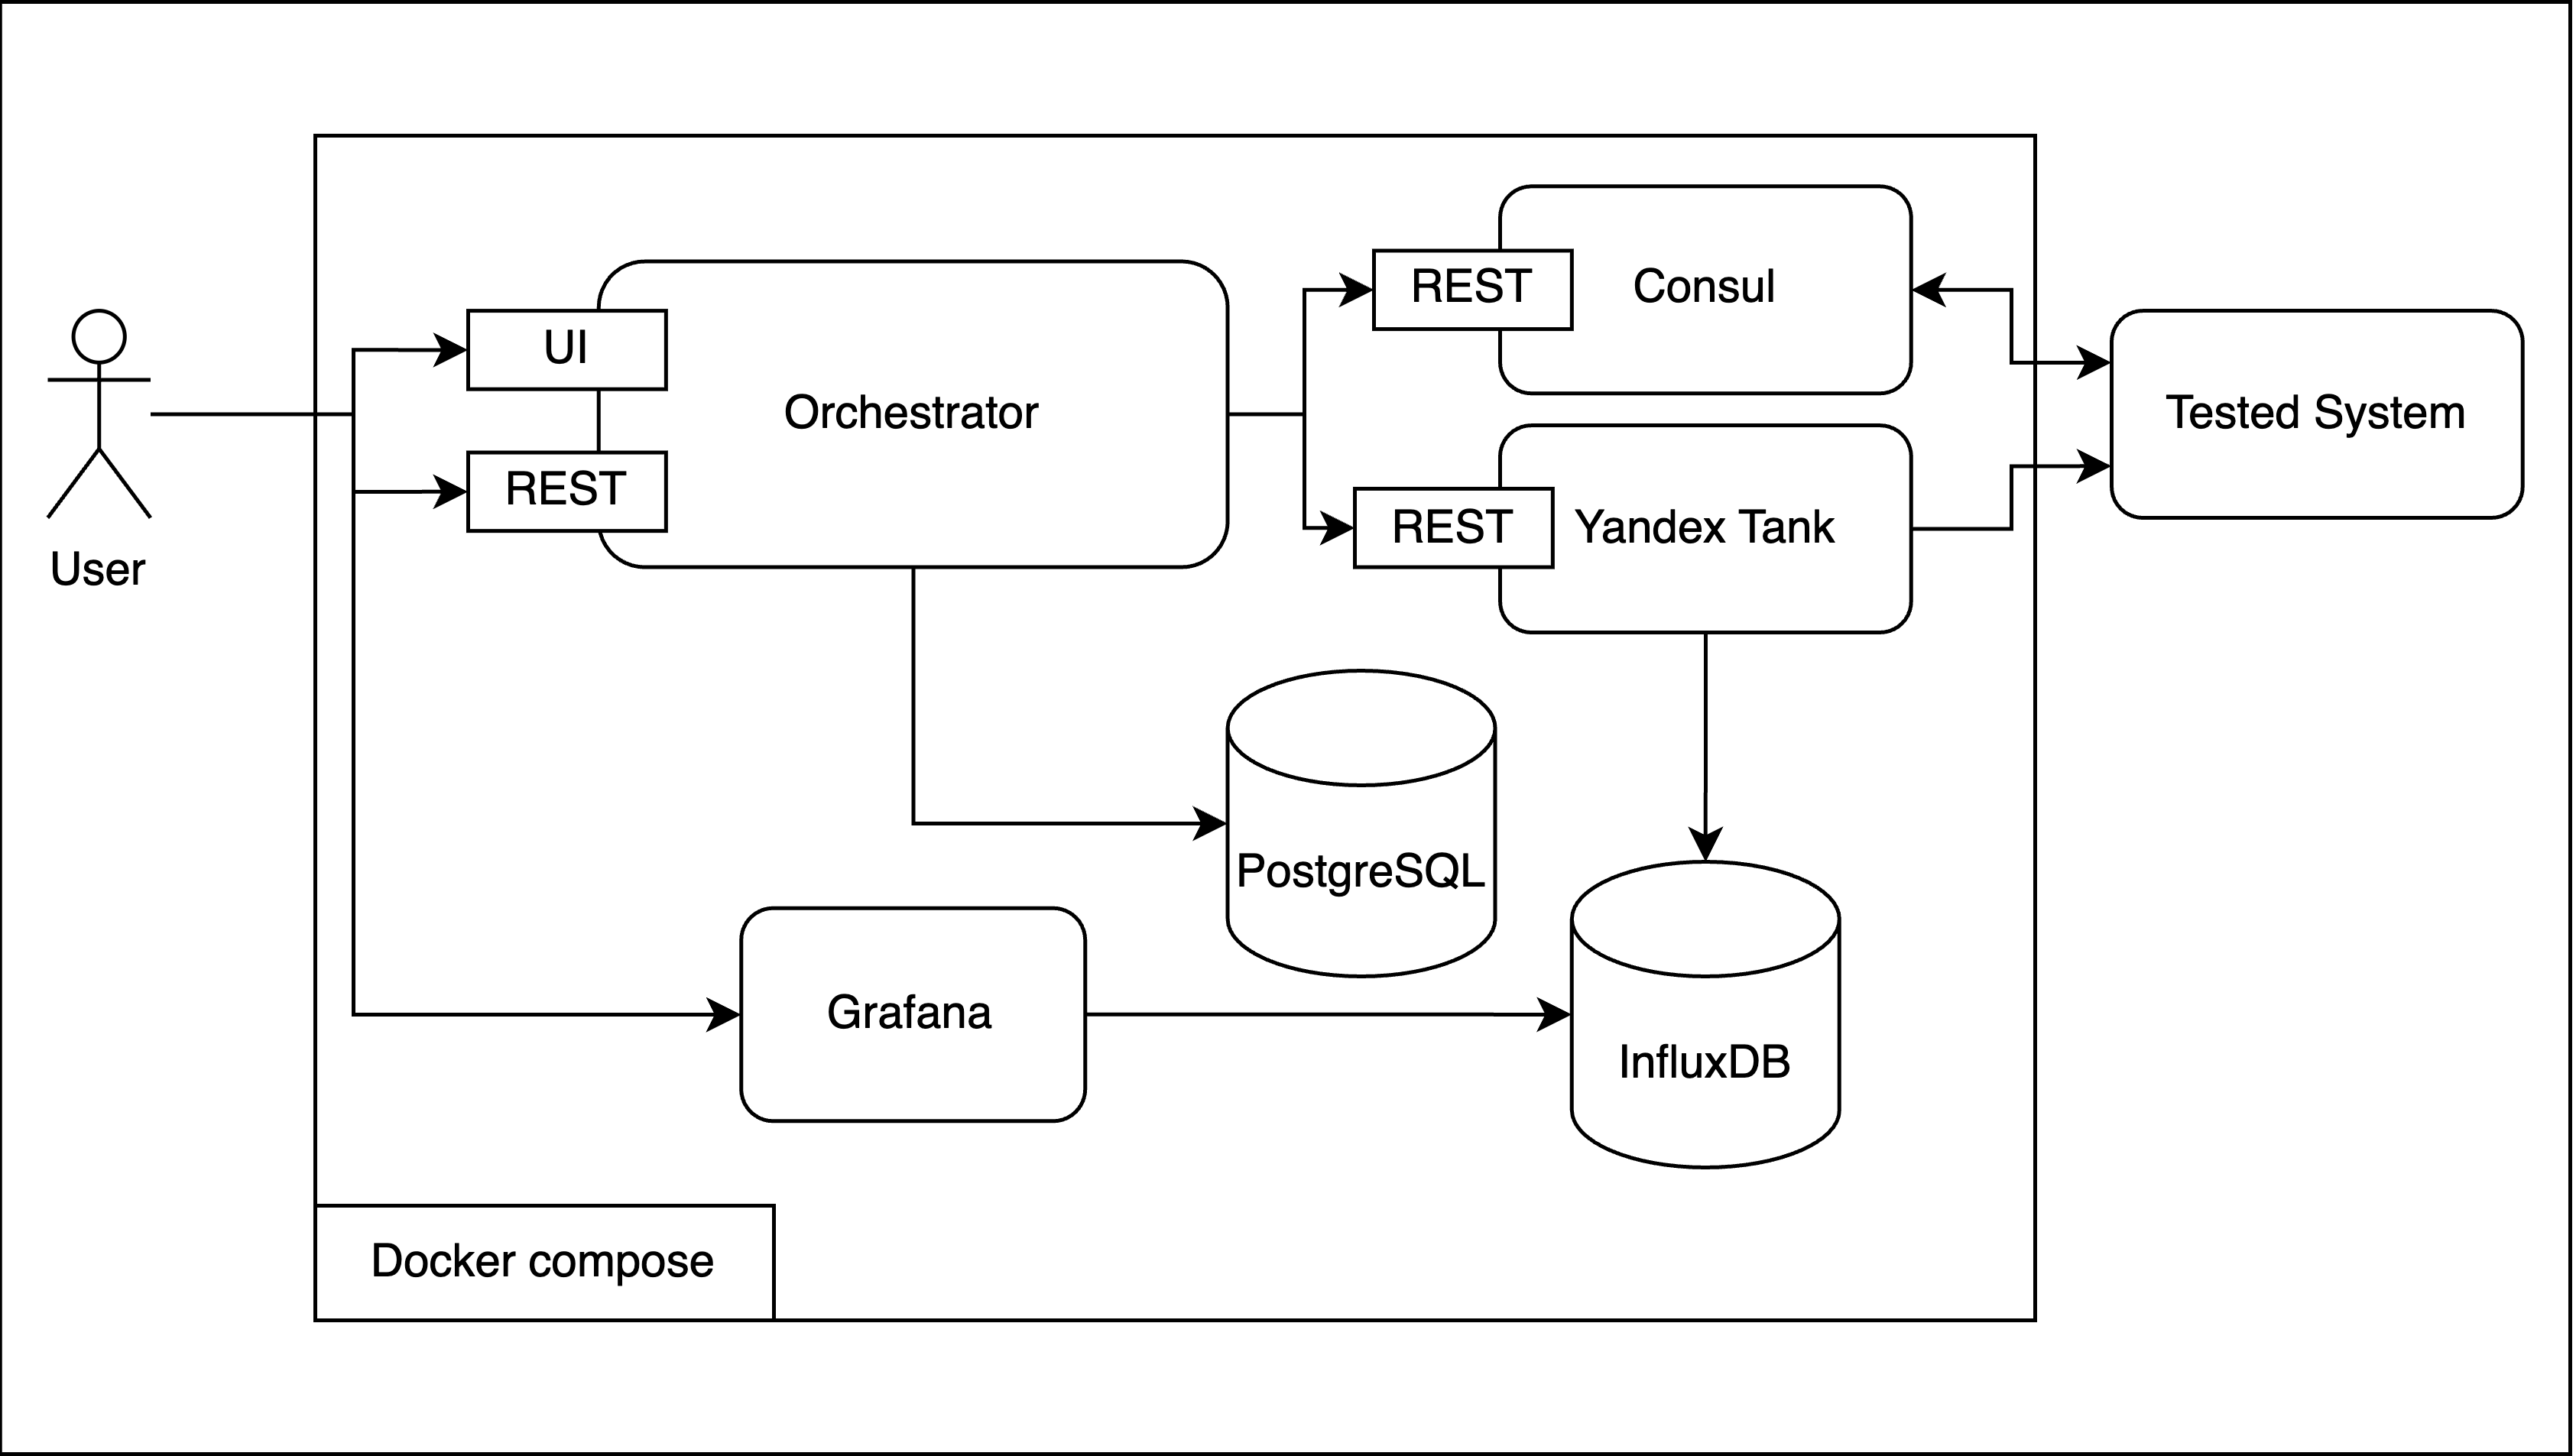
\includegraphics[height=\textheight,width=\textwidth,keepaspectratio]{architecture.png}
    \caption{Architecture of the system}
    \label{fig:architecture}
\end{figure}

\section{System Components}\label{sec:system-components}
This section discusses all the tools and technologies used in the systems, as well as the reasons why they are appropriate for the project.
\subsection{Yandex Tank API}\label{subsec:ya-api}
Yandex Tank is popular open source solution for load testing. It has convinient format of load testing configuration via YAML files. Also it can generate more the 100000 requests per seconds. But it does not provide ability to manipulate load test flow and can't be easily injected into automated web systems. Therefore, Yandex Tank API was used. It is wrapper aroung yandex tank and allows to start, stop, pause, resume load test. Additionally, it provides user-friendly REST API. All test results are saved into time series database InfluxDB described in subsection \ref{subsec:influx}

\subsection{InfluxDB}\label{subsec:influx}
The load test result is a timeline of application stats. InfluxDB is the tool that's optimized for storing that type of data. It does not require any external dependencies and it is written in Rust programming language, so it works fast. Additionaly, Yandex Tank support this database and can write results directly to it.

\subsection{PostgreSQL}\label{subsec:postgre}
For storage of load testing scenarios, history of exectutions and configuration of reliability patterns the PostgreSQL is used. This is a popular relative database management system (DBMS) that supports a wide range of data types, and the most significant for us is its support for JSON data type. In the implementation section, the entity-relationship model of the tables will be presented.

\subsection{Kafka}\label{subsec:kafka}
If a change of configuration of the reliability patterns occurs as an event, the system needs to be able to store a stream of these event. Additionally, it is needed to share this stream with the tested service, so that it can make changes to these parameters in its implementation of the pattern. A message broker system Kafka is well-suited for this purpose because it is optimized for storing stream of events.

\subsection{Grafana}\label{subsec:grafana}
Grafana is a tool used for visualizing test results. It can be integrated with InfluxDB and allows it to visualize time series data from that DBMS. Additionally, Grafana has a RESTful API that allows users to create and managed charts through HTTP requests.

\subsection{Orchestrator}\label{subsec:orchestrator}
For improved user experience, the Orchestrator User Interface (UI) is used as the primary user interface for the Orchestrator service \ref{subsec:orchestrator}. The UI provides forms for creating load test scenarios, executing load test and configuring reliability patterns. In addition, it visualises all stored scenarios, their executions and allows to change configuration of patterns.